% Companion slide deck for "A Hard-to-Beat Rule for Week-Ahead Traffic Forecasting".
% Compile: pdflatex best_rule_slides.tex  (run twice). Figures in ./figures/.
\documentclass[aspectratio=169,11pt]{beamer}
\usetheme{metropolis}
\metroset{block=fill}
\usepackage{booktabs}
\usepackage{amsmath}
\graphicspath{{figures/}}

\newcommand{\veh}{\,\text{veh/h}}
\definecolor{accent}{HTML}{2A7DE1}
\setbeamercolor{frametitle}{bg=accent}

\title{A Hard-to-Beat Rule for\\ Week-Ahead Traffic Forecasting}
\subtitle{The calendar-adjusted seasonal baseline}
\author{Traffic Forecasting Project}
\date{June 2026}

\begin{document}

\maketitle

% --------------------------------------------------------------------
\begin{frame}{The problem}
  \begin{columns}[T]
    \begin{column}{0.5\textwidth}
      Forecast hourly highway \textbf{flow} (veh/h) \textbf{one week ahead}
      (168 hours) per sensor.
      \medskip

      Key fact: traffic is \textbf{periodic with a one-week cycle} --- the same
      weekday-and-hour repeats remarkably well.
      \medskip

      \alert{Index by hour-of-week} $\phi(t)=t \bmod 168$ (day-of-week $\times$
      hour-of-day).
      \medskip

      Data: Greater Bay Area, 2{,}352 sensors, hourly, 2017--2019 (LargeST).
    \end{column}
    \begin{column}{0.5\textwidth}
      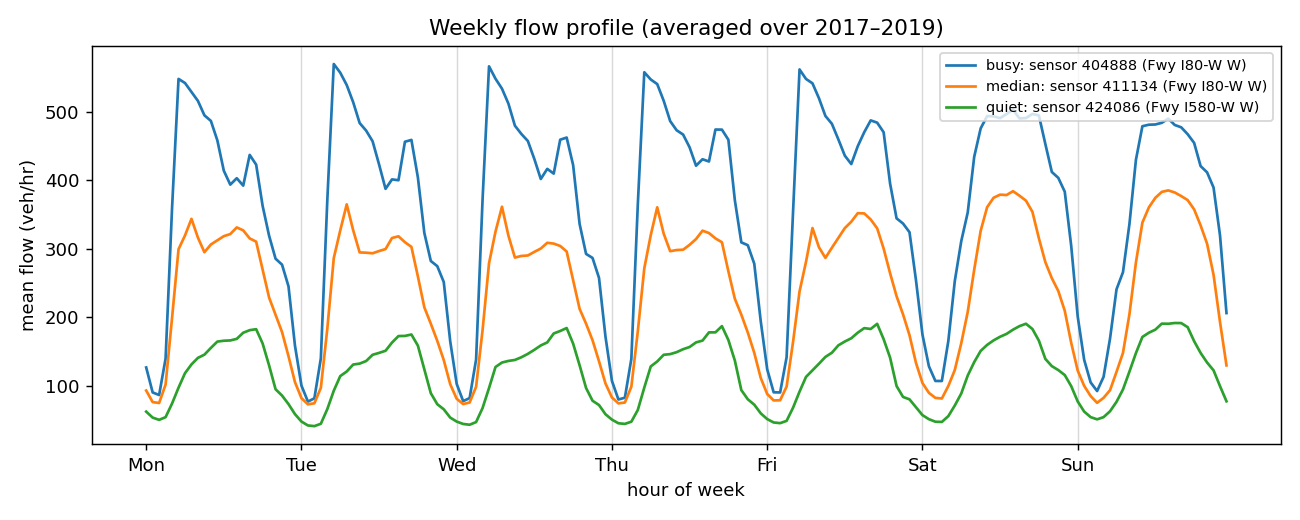
\includegraphics[width=\linewidth]{fig1_weekly_profile.png}
      \footnotesize Weekly flow profile: weekday commute double-peak, weekend hump.
    \end{column}
  \end{columns}
\end{frame}

% --------------------------------------------------------------------
\begin{frame}{The rule, in one line}
  \begin{block}{}
    \centering\large
    \textbf{Forecast} $=$ \emph{(recency-weighted average of the same hour-of-week
    over the last few weeks)} $\times$ \emph{(holiday factor on special days)}.
  \end{block}
  \vfill
  Three ingredients, building up:
  \begin{enumerate}
    \item A last-4-weeks hour-of-week \textbf{average} (the seasonal baseline)
    \item \textbf{Recency weighting} (one parameter)
    \item A \textbf{holiday/calendar factor} (known-ahead, multiplicative)
  \end{enumerate}
  \vfill
  \centering\footnotesize
  Reaches $R^2 = 0.949$, weekly-aggregate MAPE $3.55\%$ --- and we could not beat it.
\end{frame}

% --------------------------------------------------------------------
\begin{frame}{Step 1 --- last-4-weeks average (L4W)}
  Predict each hour by its recent average \emph{at the same hour of week}:
  \[
    b_t \;=\; \frac{y_{t-168} + y_{t-336} + y_{t-504} + y_{t-672}}{4}
  \]
  (lags $=1,2,3,4$ weeks). Every term is $\ge$ one week old $\Rightarrow$
  \textbf{leakage-free} for week-ahead.
  \vfill
  \begin{exampleblock}{Worked example --- next Wednesday 08:00}
    Last four Wednesdays at 08:00: $540,\,560,\,535,\,555\veh$.
    \[
      b = \tfrac14(540+560+535+555) = \mathbf{547.5}\veh
    \]
  \end{exampleblock}
  \footnotesize Averaging cancels week-to-week noise while staying recent.
\end{frame}

% --------------------------------------------------------------------
\begin{frame}{Step 2 --- recency weighting (EWMA)}
  If the level drifts, weight recent weeks more: weights $\propto \alpha^{k}$,
  $\alpha\approx0.8$, i.e. about $(0.34,\,0.27,\,0.22,\,0.17)$ recent$\to$old.
  \[
    b_t^{\text{ewma}} = 0.34\,y_{t-168} + 0.27\,y_{t-336} + 0.22\,y_{t-504}
      + 0.17\,y_{t-672}
  \]
  \begin{exampleblock}{Worked example --- a rising level}
    Last four same-hour values $500,520,540,560\veh$:
    \[
      \text{flat} = 530 \qquad\text{vs}\qquad
      \text{EWMA} = \mathbf{537.4}\veh
    \]
    EWMA leans to the recent, higher values --- tracking the drift the flat
    average lags.
  \end{exampleblock}
  \footnotesize The single decay $\alpha$ is the only ``training'' in the whole rule.
\end{frame}

% --------------------------------------------------------------------
\begin{frame}{Step 3 --- the holiday factor}
  \begin{columns}[T]
    \begin{column}{0.52\textwidth}
      The baseline's blind spot: \textbf{holidays}. It averages four \emph{normal}
      weeks and over-predicts (the commute vanishes).
      \medskip

      $8\%$ of hours, but $\sim$$23\%$ of the error --- and \textbf{known ahead}.
      \medskip

      \alert{Fix:} a multiplicative factor =
      \emph{the average, over past occurrences of that holiday, of the ratio
      $\tfrac{\text{actual}}{\text{baseline}}$ at that hour.}
      \[
        f = \tfrac12(0.70+0.72) = 0.71
      \]
      \[
        \hat y = b^{\text{ewma}} \times f
      \]
    \end{column}
    \begin{column}{0.48\textwidth}
      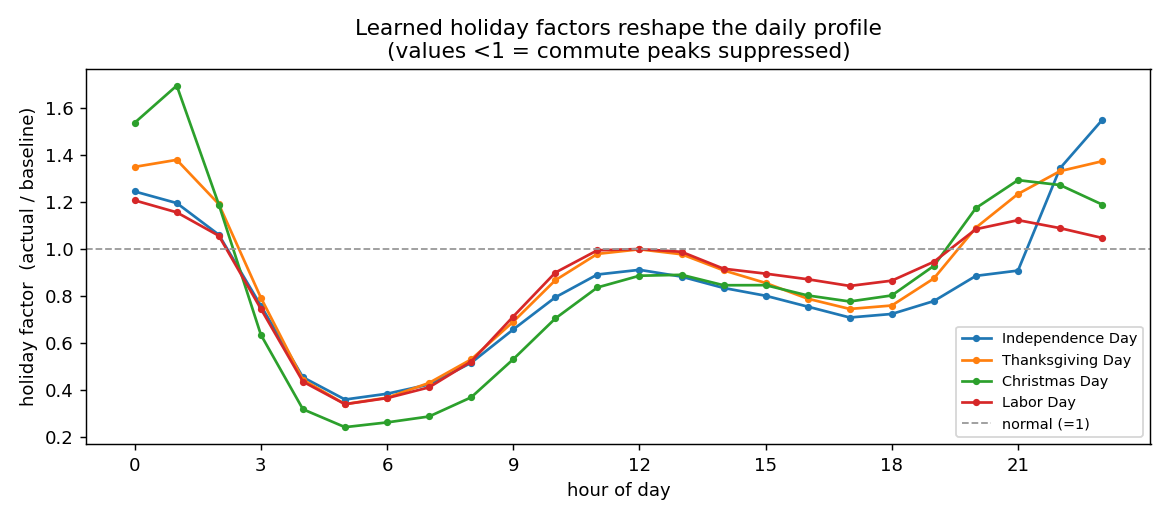
\includegraphics[width=\linewidth]{fig6_holiday_shape.png}
      \footnotesize Learned factors by hour: mornings crushed to $\sim$0.4,
      late-evening $>1$ (holiday-eve travel).
    \end{column}
  \end{columns}
\end{frame}

% --------------------------------------------------------------------
\begin{frame}{Putting it together --- a holiday, hour by hour}
  \begin{exampleblock}{July 4th at 17:00}
    baseline $490\veh \times f\,0.71 = \mathbf{348}\veh$ \quad (a $29\%$ correction)
  \end{exampleblock}
  \vfill
  \centering
  \begin{tabular}{cccc}
    \toprule
    hour & baseline (\veh) & factor $f$ & forecast (\veh) \\
    \midrule
    08:00 & 520 & 0.42 & 218 \\
    12:00 & 430 & 0.96 & 413 \\
    17:00 & 490 & 0.71 & 348 \\
    22:00 & 240 & 1.30 & 312 \\
    \bottomrule
  \end{tabular}
  \vfill
  \footnotesize Same baseline, reshaped by the learned holiday profile.
\end{frame}

% --------------------------------------------------------------------
\begin{frame}{Why it's hard to beat --- it works}
  \centering
  \begin{tabular}{lccc}
    \toprule
    Model & $R^2$ & RMSE (\veh) & RMSE on holidays \\
    \midrule
    Flat 4-week baseline       & 0.9404 & 40.14 & 66.96 \\
    \;+ recency (EWMA)         & 0.9435 & 39.10 & 65.99 \\
    \;+ holiday factor         & \textbf{0.9493} & \textbf{37.01} & \textbf{47.71} \\
    \bottomrule
  \end{tabular}
  \vfill
  \begin{itemize}
    \item Holiday factor cuts holiday-hour error \textbf{29\%} ($67\to48$),
      ordinary hours untouched.
    \item Weekly-aggregate MAPE $= \mathbf{3.55\%}$.
  \end{itemize}
\end{frame}

% --------------------------------------------------------------------
\begin{frame}{Why it's hard to beat --- it's at the ceiling}
  Best-possible \emph{in-sample} fit on the test year itself (an upper bound):
  \vfill
  \centering
  \begin{tabular}{lc}
    \toprule
    Oracle (fit on the test year) & $R^2$ \\
    \midrule
    Static hour-of-week mean        & 0.938 \\
    \; + oracle holiday effect      & 0.943 \\
    \textbf{Our out-of-sample rule} & \textbf{0.949} \\
    \bottomrule
  \end{tabular}
  \vfill
  \raggedright
  Our \emph{real} rule beats the \emph{in-sample} static oracle --- recency
  weighting tracks within-year drift a fixed mean cannot.
  \smallskip

  $\Rightarrow$ the remaining $\sim$5\% is \textbf{irreducible incident noise}.
\end{frame}

% --------------------------------------------------------------------
\begin{frame}{Why it's hard to beat --- everything fancier failed}
  \centering
  \begin{tabular}{ll}
    \toprule
    Attempt & Effect vs.\ the rule \\
    \midrule
    Autoregression on residual (hourly)   & $\le +0.003\,R^2$, decays by a week out \\
    Autoregression on weekly aggregate    & $\le +0.001\,R^2$ \\
    Ridge / XGBoost on calendar features  & $\approx 0$ (or overfits) \\
    Pooled panel AR ($+$ Fourier)         & \emph{worse} \\
    Global gradient boosting              & \emph{worse} \\
    Cross-regional common factor          & exists, but \emph{unforecastable} \\
    \bottomrule
  \end{tabular}
  \vfill
  \centering
  \alert{A one- or two-parameter rule is at the ceiling:} the signal is a
  deterministic calendar pattern; the rest is noise.
\end{frame}

% --------------------------------------------------------------------
\begin{frame}{How to improve it}
  Not with fancier models of the \emph{same} information --- only with new
  information or a new objective:
  \vfill
  \begin{enumerate}
    \item \textbf{Known-ahead covariates} --- scheduled events, planned closures
      (generalize the holiday factor; localized, help venue/corridor sensors).
    \item \textbf{Longer horizons \& more years} --- multi-week, where a slow
      \emph{level} governs error; matters from $\sim$3--4 weeks out.
    \item \textbf{Distributional forecasts} --- congestion risk, intervals; value
      in the tails, not the mean.
    \item \textbf{Harder targets} --- speed is far noisier ($R^2 \approx 0.76$).
  \end{enumerate}
\end{frame}

% --------------------------------------------------------------------
\begin{frame}[standout]
  Complexity should follow \emph{information} and \emph{objective},\\
  not precede them.
  \vfill
  \normalsize For week-ahead flow, a calendar-adjusted seasonal average\\
  is not just a baseline --- it is close to the best one can do.
\end{frame}

\end{document}
